\documentclass[a4paper]{article}
\usepackage[margin=2cm]{geometry}
\usepackage{amsmath, amssymb, graphicx, float, forloop}
\graphicspath{{../result}{../report/media}}

\begin{document}

\section{What has been done}
\begin{itemize}
    \item lines with 95\% confidence interval: system total carbon, system carbon pool, yield
    \item colour: P-only (green) \& P+B (orange)
    \item aim: plot distributions along the range for parameter-of-interest
    \item parameter hyperspace recorded in ``0619\_analysis" document
\end{itemize}

\section{graphs}
\newcounter{i}\forloop{i}{1}{\value{i}<10}{
\includegraphics[width=\linewidth]{../result/var_0\arabic{i}.png}\\\\
}
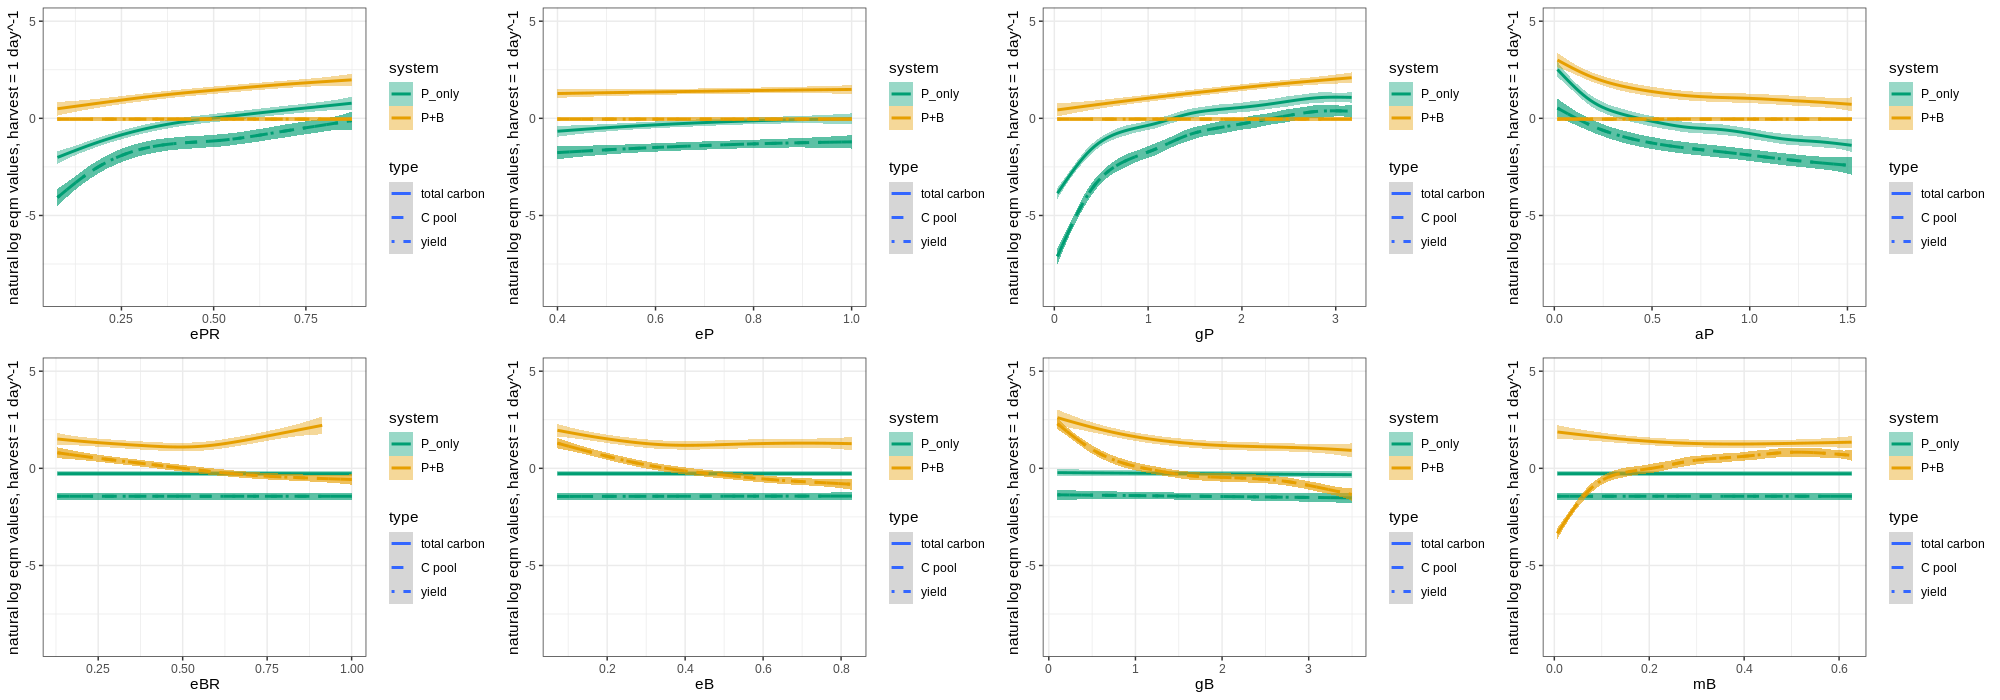
\includegraphics[width=\linewidth]{../result/var_10.png}

\end{document}